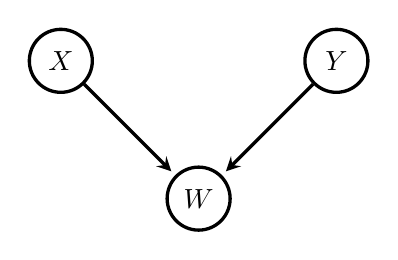
\begin{tikzpicture}[scale=3.5, 
       node/.style={circle,inner sep=1mm,minimum size=0.8cm,draw,
      very thick,black,fill=white,text=black},
        nondirectional/.style={very thick,black},
        unidirectional/.style={nondirectional,shorten >=2pt,-stealth},
        bidirectional/.style={unidirectional,bend right=10}]

	\node [node] (v1) at (-0.5, 0.5)       {$X$};
        \node [node] (v2) at (0.5, 0.5)        {$Y$};
        \node [node] (v3) at (0, 0)        {$W$};

        \path [unidirectional] (v1) edge (v3);
        \path [unidirectional] (v2) edge (v3);
\end{tikzpicture}
